\documentclass{article}

% Packages
\usepackage{amsmath}    % For math formatting
\usepackage{graphicx}   % For images/figures
\usepackage{geometry}   % Page layout
% \usepackage{fancyhdr}   % Custom headers/footers
\usepackage{titling}    % Title customization
\usepackage{hyperref}   % Table of Contents links
\usepackage{lipsum}     % Placeholder text
\usepackage{caption}    % Caption for tables and figures

% Page numbering on specific pages
% \pagestyle{fancy}
% \fancyhf{}
% \fancyfoot[C]{\thepage}

% Custom settings to control page numbers
\pagenumbering{gobble} % No page numbers on the title and TOC pages
\newcommand{\startPageNumbering}{\pagenumbering{arabic}\setcounter{page}{1}} % Start page numbering on page 3

% Title information
\title{My First LaTex Article}
\author{Baiyi Lian}
\date{\today}

\begin{document}

% Title page
\maketitle
\newpage

% Table of Contents
\tableofcontents
\newpage

% Start page numbering
\startPageNumbering

% Section 1: Maths
\section{Maths}
\subsection{Pythagorean Theorem}
In the Pythagorean equation $c^2 = a^2 + b^2$ \textbf{a} and \textbf{b} represent lengths of a triangle's two sides and \textbf{c} the length of the hypotenuse. Equations can also be centered:
\[
\centering
f(x) = x^2
\]

% Section 2: Figure
\section{Figure}

\begin{figure}[h!]
    \centering
    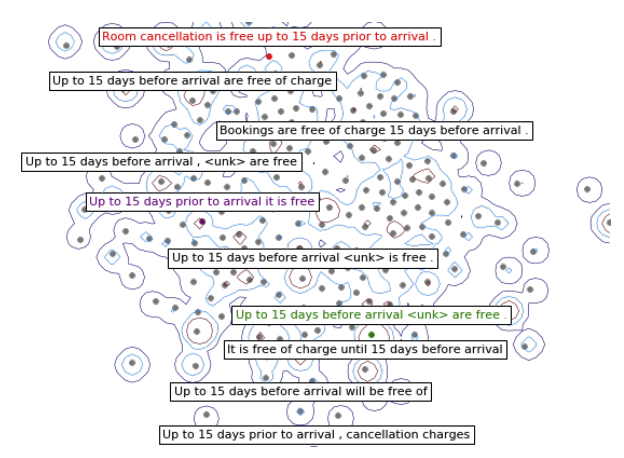
\includegraphics[width=0.6\textwidth]{figure1.png} % Replace with the path to your image
    \caption{Visualization of sequence-level interpolation on an
example German → English sentence \cite{kim-rush-2016-sequence}.}
    \label{fig:seq}
\end{figure}

% Section 3: Table
\section{Table}

\begin{table}[h!]
    \centering
    
    \begin{tabular}{c|c}
        \hline
        Model & BLEU \\
        \hline
        Baseline & 14.7 \\
        \hline
        Word-KD & 15.4 \\
        \hline
        Seq-KD & 18.9

    \end{tabular}
    \caption{Results on English-German (newstest2014) and Thai-English (2012/2013) test sets.}
\end{table}

% Section 4: Referencing
\section{Referencing}
When referencing in a text, you can use a BibTex generator.\newline
Here I add a reference to the figure\cite{kim-rush-2016-sequence} used. Using BibTex I get a reference list created in the end of the document.

\bibliographystyle{plain}
\bibliography{reference}

\end{document}
